\chapter{Environments' Details}
\label{sec:environments-details}
The sections of this chapter provide additional details about the custom environments used in our experiments.
Both of these environments were developed in Python.

\section{ShapeGridWorld}
\label{sec:sgw-details}
% Added color
% Added object_persistency 0
% Added step_size > 1
% Improved rendering
% Added partial reset with control and control boundaries
% Added controlled reset with max_dist
% Added partial control with control and control boundaries
\tabref{tab:original-sgw-params} lists the parameters of the original ShapeGridWorld environment developed by \cite{rair}.
\begin{table}[H]
    \centering
    \begin{tabularx}{\textwidth}{C{3.9cm} L}
        \hline
        Property & Description\\
        \hline
        \texttt{width} & Width of the discrete grid.\\
        \texttt{height} & Height of the discrete grid. Kept same as \texttt{width}.\\
        \texttt{n\_pixels} & Number of ``On'' pixels.\\
        \texttt{shape} & Shape of a pixel block -- ``circle''.\\
        \texttt{size} & Size of a pixel block.\\
        \texttt{persistency} & Number of time steps an object (pixel block) is moved. \\
        \hline
    \end{tabularx}
    \caption{Original ShapeGridWorld parameters.}
    \label{tab:original-sgw-params}
\end{table}
The state space of this environment is composed of the \(x\) and \(y\) coordinates of the \(n\) block pixels, with the addition of two dimensions -- one that specifies which object is currently in focus and another that specifies how many times it has already moved, i.e. \(\cS \in \nN^{2 n + 2}\).
The observation space is a rendering of the grid as an image of shape \(\texttt{width} * \texttt{size} \times \texttt{height} * \texttt{size}\).

The action space comprises the action value for each of the directions (x and y) for an object; \(\cA \in [-1, 1]^{2 n}\).
For each dimension, the controller samples from a continuous distribution in \([-1, 1]\), which is uniformly mapped to \(\{-1, 0, 1\}\) (\([-1, -1/3) \mapsto -1, [-1/3, 1/3] \mapsto 0, (1/3, 1] \mapsto 1\)).

We further added more features to this environment for our experiments, which are listed in \tabref{tab:additional-sgw-params}.
In particular, the ability to move all objects at once and more than one step in an action step was added.
We also developed a controlled reset method with the added feature to freeze sections of the grid, with \texttt{control} and \texttt{control\_boundaries}.
This additionally enabled us to allow the controller only partial access to the environment.
Furthermore, the rendering function was reimplemented using faster methods from \emph{OpenCV}; see \secref{sec:improving-render} for more details.

\begin{table}[h]
    \centering
    \begin{tabularx}{\textwidth}{C{3.9cm} L}
        \hline
        Property & Description\\
        \hline
        \texttt{step\_x} & Maximum number of steps an object can be translated in the x-direction in one action.\\
        \texttt{step\_y} & Maximum number of steps an object can be translated in the y-direction in one action. Kept same as \texttt{step\_x}.\\
        \texttt{persistency*} & Added the ability to move all objects at once.\\
        \texttt{color} & A flag that indicates if pixels should have a grayscale value. \\
        \texttt{invert} & A flag to control the inversion of the rendered images. \\
        \texttt{control\_boundaries} & If specified, objects inside these limits \emph{initially} are marked.\\
        \texttt{control} & A flag that indicates whether the controller can move all the objects or those marked initially by the control boundaries.\\
        \texttt{max\_reset\_dist} & Maximum distance an object can be moved from its original position on reset. Only the objects marked initially are reset (default: \(5\)).\\
        \hline
    \end{tabularx}
    \caption{Additional ShapeGridWorld parameters.}
    \label{tab:additional-sgw-params}
\end{table}

If all objects are moved at once, the state space of this environment is composed of only the \(x\) and \(y\) coordinates of the block pixels, i.e. \(\cS \in \nN^{2 n}\).
The corresponding action space in this case would be \(\cA \in [-1, 1]^{2 n}\).
For each dimension of the action space, the controller samples from a continuous distribution in \([-1, 1]\), which is uniformly mapped to integers \([-l, l]\), where \(l \in \{\texttt{step\_x}, \texttt{step\_y}\}\) is the step size of the dimension.

\subsection{ShapeGridWorld Image Registration Technique}
\label{sec:sgw-registration}

To test CLIP inference on ShapeGridWorld and simulate the controller on partial drawings, without having to draw these drawing samples manually, a registration method for images was developed that reads a given image to generate a corresponding ShapeGridWorld of given dimensions.

This is done using a circular convolution kernel over the image to find the corresponding grid pixel values.
Optionally, it makes the lines in the image thinner by finding its skeleton using morphological operations before the convolution.
See \figref{fig:sgw-registration} for a demonstration.

\vspace{10pt}
\begin{figure}[h]
    \centering
    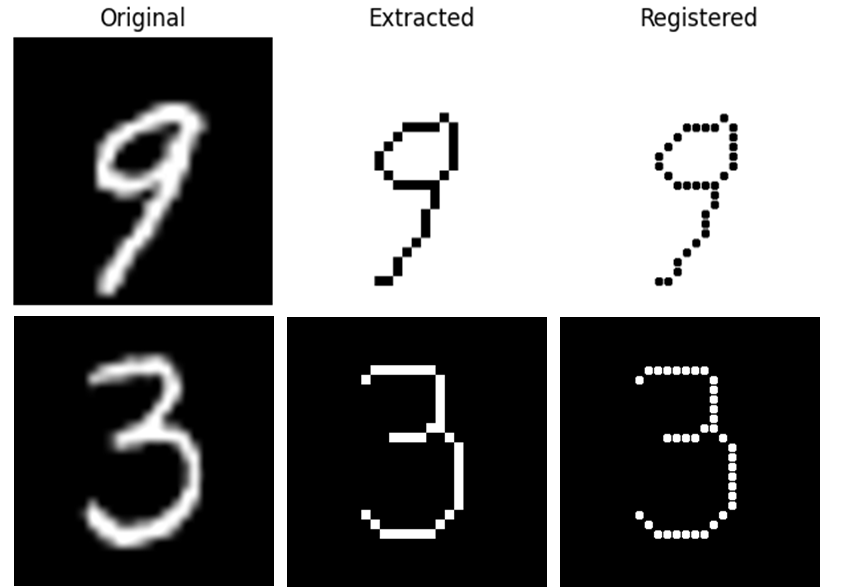
\includegraphics[width=0.6\textwidth]{images/grid_registration.png}
    \caption{ShapeGridWorld image registration on images from the MNIST dataset.}
    \label{fig:sgw-registration}
\end{figure}

\vspace{10pt}
We developed a wrapper around the PIL Python library \citep{pil} to conveniently perform these operations and generate ShapeGridWorld environments.
The relevant code is hosted on \url{https://github.com/pulkitgoyal56/ImageGrid}.
\tabref{tab:imagelib-params} lists the relevant parameters of this image registration library.
\begin{table}[h]
    \centering
    \begin{tabularx}{\textwidth}{C{3.9cm} L}
        \hline
        Property & Description\\
        \hline
        \texttt{mode} & PIL Image mode in which the image is read.\\
        \texttt{invert} & A flag to control the inversion of the read image. \\
        \texttt{threshold\_ratio} & Threshold on the convolution sum, for binary grids with no color.\\
        \hline
    \end{tabularx}
    \caption{Image registration parameters.}
    \label{tab:imagelib-params}
\end{table}


\newpage
\section{Tangram}
\label{sec:tangram-details}
% flip
% rotate
% x_size
% r_size
% x_step
% object_persistency
% max_dist
% control
% control_boundaries
% staging_boundaries

The Tangram environment is initialized with a list of polygon objects created using the provided \texttt{Polygon} class, which defines a polygon's size, shape, and color.
The additional parameters of the Tangram environment are tabulated in table \tabref{tab:tangram-params}.
\begin{table}[H]
    \centering
    \begin{tabularx}{\textwidth}{C{3.9cm} L}
        \hline
        Property & Description\\
        \hline
        \texttt{x\_size, y\_size} & Span of the discrete grid; number of steps in the x and y directions. If set to \(1\), grid is continuous in \([0, 1]\) (default: \texttt{y\_size} = \texttt{x\_size}).\\
        \texttt{x\_step, y\_step} & Maximum number of steps a polygon can be translated in the x and y directions in one action (default: \texttt{y\_step} = \texttt{x\_step}).\\
        \texttt{r\_size} & Span of the discrete grid; number of rotation steps in \(180^\circ\). If set to \(1\), rotation is continuous in \([0, 180^\circ]\).\\
        \texttt{r\_step} & Maximum number of steps a polygon can be rotated in one action.\\
        \texttt{rotate} & A flag to enable/disable rotation.\\
        \texttt{flip} & A flag to enable/disable flipping.\\
        \texttt{persistency} & Number of time steps a polygon (pixel block) is moved. If set to \(1\), all polygons are moved at once.\\
        \texttt{control\_boundaries} & If specified, polygons inside these limits \emph{initially} are marked (default: NA).\\
        \texttt{control\_criteria} & The point inside the polygon that determines if the polygon is inside or outside the control boundaries. A Python lambda function or an attribute of \texttt{Polygon}, such as ``centroid'', ``center'', or ``complete'' (default: ``center'').\\
        \texttt{control} & A flag that indicates whether the controller can move all the polygons or those marked initially by the control boundaries (default: ``all'').\\
        \texttt{staging\_boundaries} & If specified, only polygons inside these limits are rendered to get the state's corresponding image observation (default: NA).\\
        \texttt{staging\_criteria} & Similar to \texttt{control\_criteria} but for staging boundaries (default: ``complete'').\\
        \texttt{max\_reset\_dist} & Maximum distance a polygon can be moved from its original position on reset. Only the polygons marked initially are reset (default: \(-1\); no constraints).\\
        \hline
    \end{tabularx}
    \caption{Tangram parameters.}
    \label{tab:tangram-params}
\end{table}

The state space of this environment is composed of the \(x\) and \(y\) coordinates of the vertices of the \(n = 7\) polygons, with the addition of two dimensions -- one that specifies which polygon is currently in focus and another that specifies how many times it has already moved, i.e. \(\cS \in \nN^{\,2 + \sum_{i \in n} 2\ n_v(p_i)}\), where \(n_v(p_i)\) is the number of vertices of polygon \(p_i\).
If all polygons are moved at once, the state space of this environment is composed of only the \(x\) and \(y\) coordinates of the block pixels, i.e. \(\cS \in \nN^{\sum_{i \in n} 2\ n_v(p_i)}\).
The observation space is a rendering of the grid whose resolution is controlled with different parameters.

The action space comprises the action value for each of the degrees of freedom (x, y, rotation, and flip) for an object; \(\cA \in [-1, 1]^4\).
For each dimension of the action space, the controller samples from a continuous distribution in \([-1, 1]\).
In the x-, y-, and rotation dimensions, this is uniformly mapped to integers in \([-l, l]\), where \(l \in \{\texttt{step\_x}, \texttt{step\_y}, \texttt{step\_r}\}\) is the step size of the dimension, if it is discrete.
If the dimension is continuous (because its \texttt{size} is set to \(1\)), the action is scaled by its respective step size instead.
For example, if \texttt{x\_size} is \(1\) and \texttt{x\_step} is \(3\), the resulting support of the action distribution for any action sampled for x-dimension will be \([-1/3, 1/3]\).
For the flip dimension, the mapping is (\([-1, 0] \mapsto \texttt{False}, (0, 1] \mapsto \texttt{True}\)).

The developed code to create Tangram-like environments with any number of arbitrary convex polygons is available on \url{https://github.com/pulkitgoyal56/Tangram}.

\newpage
\begin{figure}[H]
    \centering
    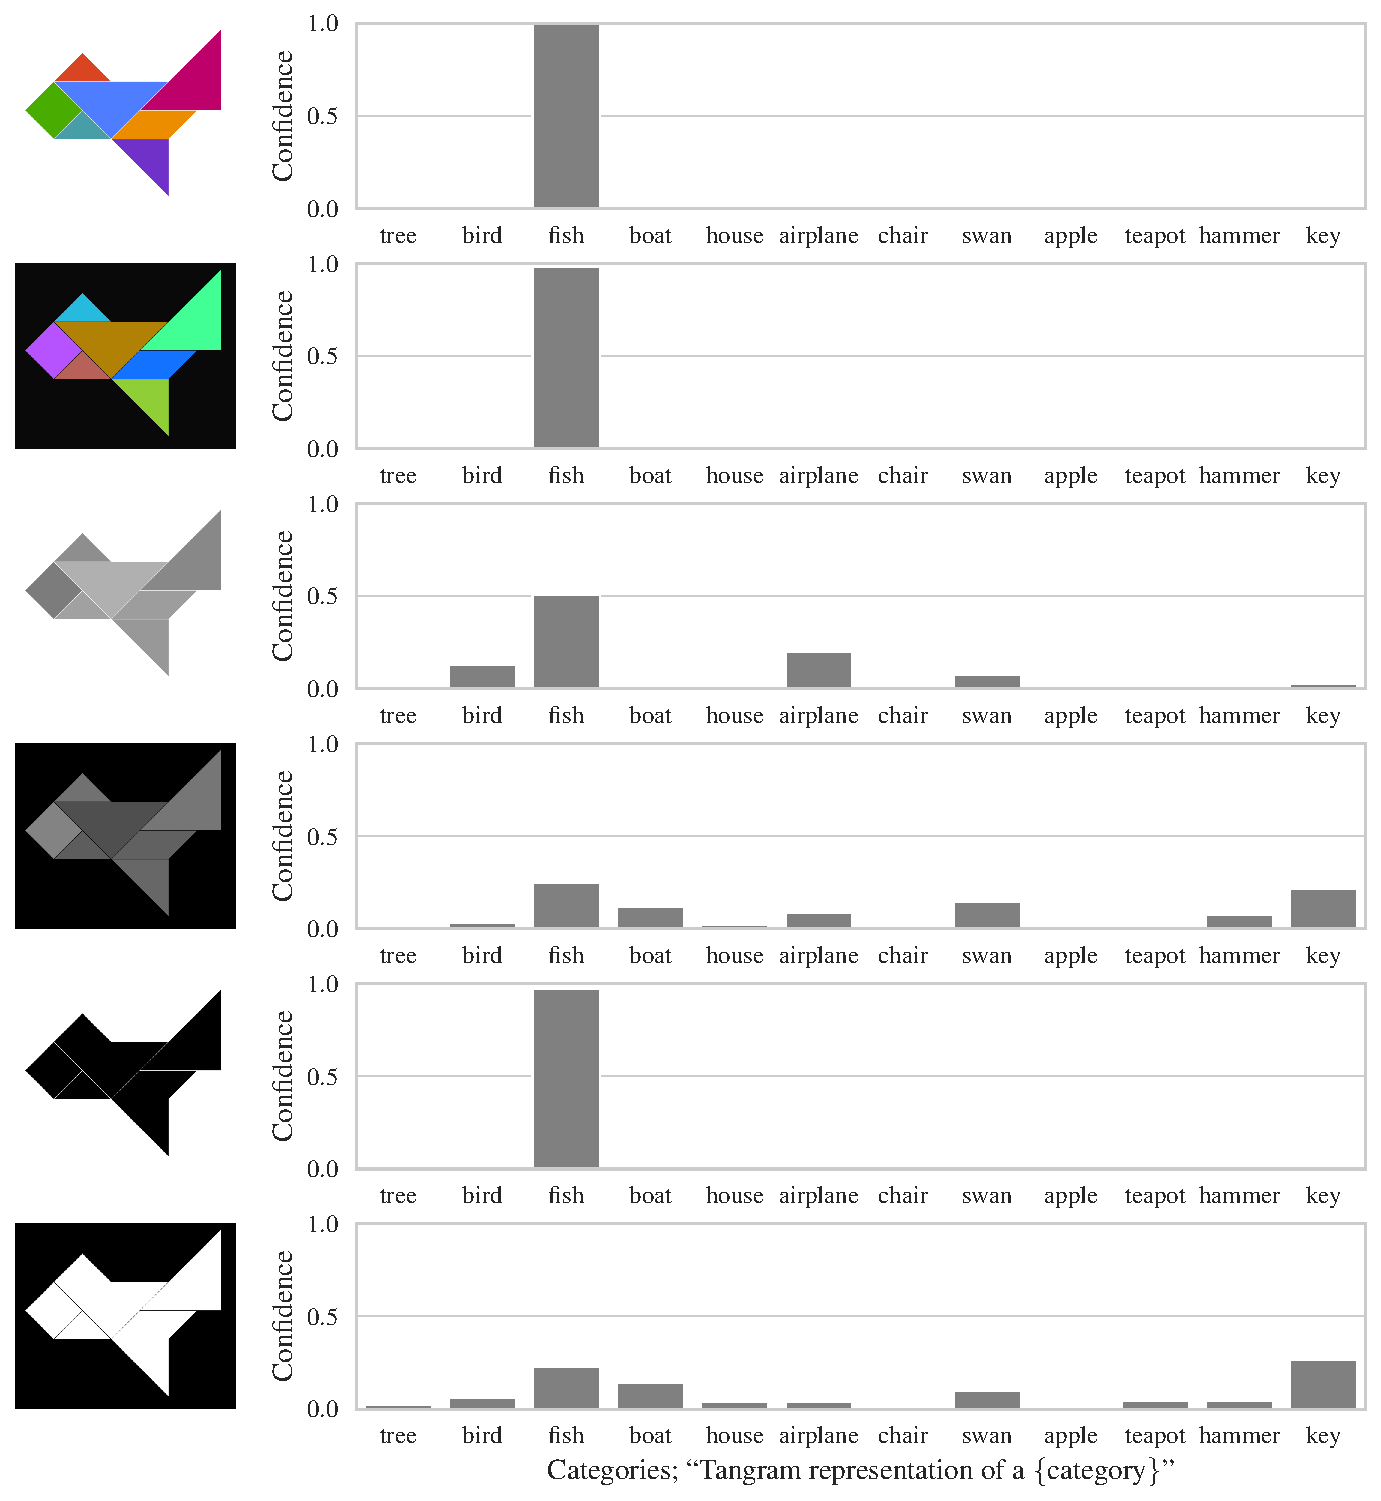
\includegraphics[width=\textwidth]{images/tangram_fish_10.pdf}
    \caption{CLIP on different inversions of the same Tangram creations. \(T = 0.1\).}
    \label{fig:clip-tangram-inversions}
\end{figure}


\chapter{Controller Hyperparameters}
\label{sec:icem-details}
% task_horizon
% horizon
% num_simulated_trajectories
% cost_along_trajectory
% action_sampler_params.opt_iterations
% action_sampler_params.init_std
% action_sampler_params.elites_size
% discount_along_trajectory
The iCEM controller introduced in \secref{sec:icem} has several hyperparameters that need to be tuned for optimal performance.
\tabref{tab:icem-params} lists the hyperparameters we tweaked in our experiments.

\begin{table}[H]
    \centering
    \begin{tabularx}{\textwidth}{C{4.7cm} L}
        \hline
        Property & Description\\
        \hline
        \texttt{horizon} & Number of steps in the future to plan, \(h\).\\
        \texttt{n\_trajectories} & Number of trajectories to sample, \(n\).\\
        \texttt{cost\_along\_trajectory} & Cost/reward aggregation function to evaluate the trajectory, \(g\). See \secref{sec:reward-aggregation} for explanations.\\
        \texttt{n\_inner\_iterations} & Number of iterations for the inner optimization loop, \(m\).\\
        \texttt{init\_std} & Standard deviation at which the sampling distribution is initialized, \(\bmsigma_0\).\\
        \texttt{elites\_size} & Size of the elite set, \(K\). See eq. \eqref{eq:icem-filter}.\\
        \texttt{discount\_factor} & Discount factor for returns expected in the future, \(\gamma\). See eq. \eqref{eq:reward-aggregation-sum-discount} (default: \(1.0\); pink noise).\\ 
        \hline
    \end{tabularx}
    \caption{iCEM controller parameters.}
    \label{tab:icem-params}
\end{table}

The other important hyperparameters that we did not tweak in our experiments are listed in \tabref{tab:icem-params-fixed}.

% factor_decrease_num: 1
% alpha: 0.1
% relative_init: true
% keep_previous_elites: true
% shift_elites_over_time: true
% fraction_elites_reused: 0.3
% use_mean_actions: true
% noise_beta: 3.5

\todo[color=red]{check and complete this}
\begin{table}[H]
    \centering
    \begin{tabularx}{\textwidth}{C{4.7cm} L}
        \hline
        Property & Description\\
        \hline
        \texttt{factor\_decrease\_num} & \\
        \texttt{alpha} & Momentum term for updating parameters of the sampling distribution.\\
        \texttt{relative\_init} & \\
        \texttt{keep\_previous\_elites} & A flag to enable passing elites to the next timestamp (outer iteration).\\
        \texttt{shift\_elites\_over\_time} & A flag to enable passing elites over inner iterations.\\
        \texttt{fraction\_elites\_reused} & Fraction of passed elites from the previous inner/outer iteration added to the sampled trajectory set.\\
        \texttt{use\_mean\_actions} & If the mean of the sampling distribution is appended to the elite set at the end of inner iterations.\\
        \texttt{noise\_beta} & Colored noise exponent of the distribution, \(\beta\) (default: \(1\)).\\
        \hline
    \end{tabularx}
    \caption{iCEM controller fixed parameters.}
    \label{tab:icem-params-fixed}
\end{table}

Please refer to the original paper for more details on the parameters of iCEM.


\chapter{Reward Hyperparameters}
\label{sec:reward-details}

This chapter lists the hyperparameters of the reward functions used in our experiments.

\section{Semantics Reward}
\label{sec:semantics-reward-details}

\subsection{Semantics Entropy Reward}
\label{sec:semantics-entropy-reward-details}
% label_prefix
% label_suffix
% categories
% semantics_baseline
% semantics_image_baseline
% semantics_alpha_target
% semantics_beta_image
% semantics_model_temperature
% semantics_model_version
% semantics_normalize
% semantics_reward_scale

\tabref{tab:entropy-reward-params} lists the parameters of the regularized semantics entropy reward from eq. \eqref{eq:entropy-reward-reg}.
\begin{table}[H]
    \centering
    \begin{tabularx}{\textwidth}{C{3.9cm} L}
        \hline
        Property & Description\\
        \hline
        \texttt{categories} & List of creative possibilities, \(\bml\).\\
        \texttt{label\_prefix} & Prefix to be added to the categories to create text labels.\\
        \texttt{label\_suffix} & Suffix to be added to the categories to create text labels.\\
        \texttt{baseline} & Baseline text input, \(\bfl_b\).\\
        \texttt{image\_baseline} & Baseline image input, \(\bfi_b\).\\
        \texttt{alpha\_target} & Regularization parameter for target text, \(\alpha\).\\
        \texttt{beta\_image} & Regularization parameter for input image observation, \(\beta\).\\
        \texttt{model\_version} & Name of the CLIP variant used.\\
        \texttt{model\_temperature} & Temperature for the softmax function in the semantics entropy reward, \(T\).\\
        \texttt{normalize} & If the reward should be normalized by maximum entropy, \(\log(|\bml|)\) (default: True).\\
        \texttt{reward\_scale} & Factor with which the reward is scaled. Together with the \texttt{reward\_scale} for the regularity reward, this determines the reward ratio, \(\lambda\) from eq. \eqref{eq:semantics-reward} (default: \(1\)).\\
        \hline
    \end{tabularx}
    \caption{Semantics entropy reward parameters.}
    \label{tab:entropy-reward-params}
\end{table}


\subsection{Regularity Reward}
\label{sec:regularity-reward-details}
% compression_precision
% compression_granularity
% compression_bidirectional
% compression_normalize
% compression_reward_scale

In the introduction to the regularity reward in \secref{sec:regularity-reward}, we mentioned the additional hyperparameters \(h\) -- \emph{resolution} and \emph{bidirectionality}.
This section provides more details about these hyperparameters.

The hyperparameter for resolution consists of two parts -- precision and granularity.
Equation \eqref{eq:rair-relational-extended} extends eq. \eqref{eq:rair-relational} with these hyperparameters to define the \(\lfloor \cdot \rceil\) operator.
\begin{equation}
    \lfloor s^{(j)} - s^{(k)} \rceil = \begin{cases}\begin{aligned}
        \left\lfloor \left| s^{(j)} - s^{(k)} \right| \frac{\text{precision}}{\text{granularity}} \right\rfloor \times \text{granularity} &\text{if bidirectionality} = \text{False}\\
        \left\lfloor \left( s^{(j)} - s^{(k)} \right) \frac{\text{precision}}{\text{granularity}} \right\rfloor \times \text{granularity} &\text{if bidirectionality} = \text{True}\\
    \end{aligned}\end{cases}
    \label{eq:rair-relational-extended}
\end{equation}
\tabref{tab:regularity-reward-params} lists the parameters of the regularity reward.
\begin{table}[H]
    \centering
    \begin{tabularx}{\textwidth}{C{3.9cm} L}
        \hline
        Property & Description\\
        \hline
        \texttt{precision} & Precision of the compression algorithm.\\
        \texttt{granularity} & Granularity of the compression algorithm.\\
        \texttt{bidirectional} & If the compression should be bidirectional.\\
        \texttt{normalize} & If the reward should be normalized by the maximum possible entropy, \(\log\left(\binom{N}{2}\right)\) (default: True).\\
        \texttt{reward\_scale} & Factor with which the reward is scaled. Together with the \texttt{reward\_scale} for the semantics entropy reward, this determines the reward ratio, \(\lambda\) from eq. \eqref{eq:semantics-reward}.\\
        \hline
    \end{tabularx}
    \caption{Regularity reward parameters.}
    \label{tab:regularity-reward-params}
\end{table}

Please refer to the original paper for more details on the theory and implementation of \emph{RaIR}.

\section{Closeness Reward}
\label{sec:closeness-reward-details}
% closeness_reward_type
% closeness_reward_scale
% closeness_reward_threshold

\tabref{tab:closeness-reward-params} lists the parameters of the closeness reward from \secref{sec:closeness-rollouts}.
\begin{table}[H]
    \centering
    \begin{tabularx}{\textwidth}{C{3.9cm} L}
        \hline
        Property & Description\\
        \hline
        \texttt{reward\_type} & Type of closeness reward -- \emph{sparse-incremental} or \emph{dense}.\\
        \texttt{reward\_scale} & Factor with which the reward is scaled.\\
        \texttt{reward\_threshold} & Threshold, \(\varepsilon\), for sparse rewards, eq. \eqref{eq:closeness-reward-sparse}.\\
        \hline
    \end{tabularx}
    \caption{Closeness reward parameters.}
    \label{tab:closeness-reward-params}
\end{table}


\chapter{Comparing CLIP Models}
\label{sec:clip-comparison}

The vision transformer (ViT) models have better accuracy than Resnet models.
Resnet models have a gradual slope in rollouts compared to ViT models and flatter distributions on random images.

\begin{figure}[h]
    \centering
    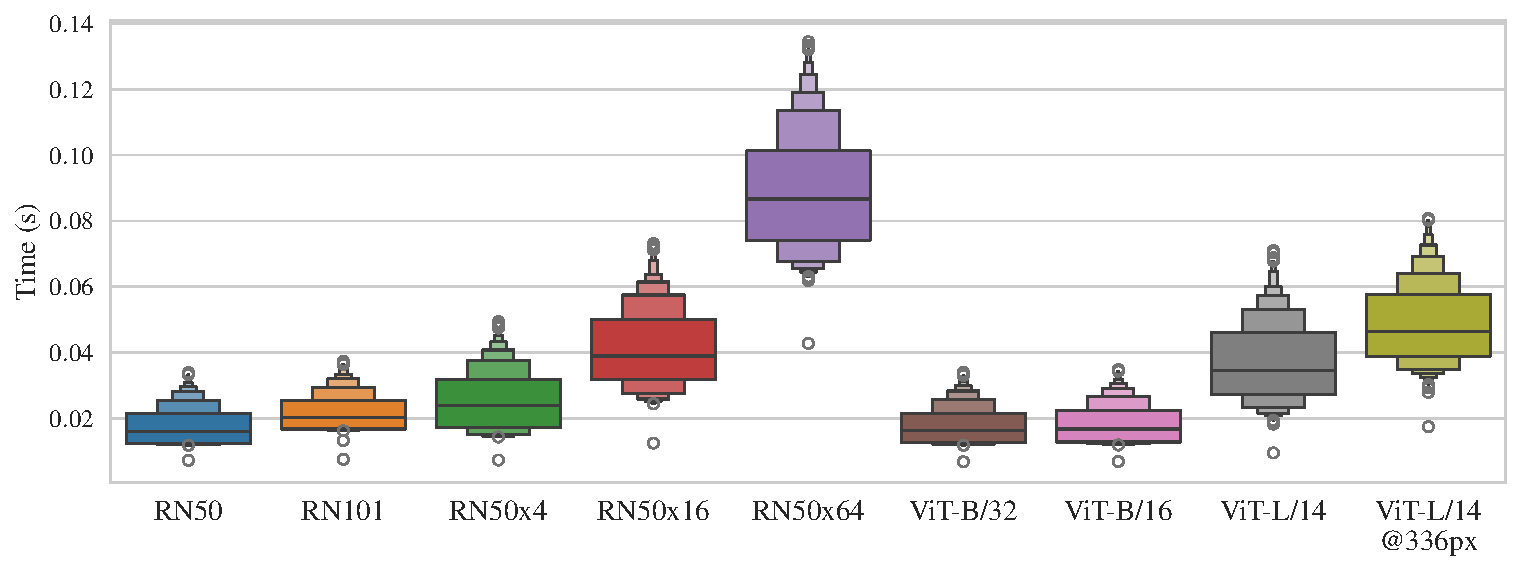
\includegraphics[width=\textwidth]{images/clip_inference_times.pdf}
    \caption{Comparing times of different original CLIP models for embedding a single image.}
    \label{fig:clip-comparison}
\end{figure}


\chapter{Flatnet}
\label{sec:flatnet}
To test the feasibility and efficacy of fine-tuning CLIP with an entropy regularization technique (eq. \ref{eq:entropy-regularization}) to reduce its inference noise, we conducted experiments on a smaller toy setup with convolutional neural networks trained as an number classifier on ShapeGridWorld images using the MNIST dataset.
We additionally augmented the MNIST training dataset with samples of images with random arrangements of pixels, labelled with an uniform distribution of confidence over the output of the model.

We treated the entropy regularization strength and the addition of random samples as hyperparameters and trained a series of models with different combinations of the two.
\figref{fig:flatnet-comparison} shows the resulting trajectories over the 

\begin{figure}[h]
    \centering
    \missingfigure{Flatnet comparison over the 495 closeness trajectory}
    \caption{Comparing times of different original CLIP models for embedding a single image.}
    \label{fig:flatnet-comparison}
\end{figure}

% \chapter{Descriptive List of Main Hyperparameters}
% \label{sec:hyperparameters}
% Here, we provide a list of the hyperparameters we mainly considered in our experiments.


\chapter{Improving Simulation Times}
\label{sec:efficiency}
Rendering the environment and using CLIP for planning was a very resource-intensive operation.
At every planning step, a total of \(\text{n\_trajectories} \times \text{horizon} \times \text{n\_icem\_inner\_iterations}\) evaluations needed to be computed.
This was further multiplied by the number of steps in the simulation.
This total ranged anywhere from \(~200,000\) to \(~2,000,000\) in our many experiments which corresponded to about \(2\) to \(20\) hours of simulation time if run in a single batch of inference on multiple GPUs.

Reducing simulation time was critical for us to be able to do any hyperparameter analysis.
We implemented several optimization techniques to improve this, which mainly involved efficient \emph{vectorization} of all computations, lazy evaluation, caching, parallelization, and cutting down on redundant operations.
In particular, two of these, for rendering and inference, are briefly introduced in the following sections.

\section{Reducing Rendering Time}
\label{sec:improving-render}
The rendering time was a major bottleneck for the simulations.
To improve this, we experimented with three popular open-source graphics Python libraries; \emph{Matplotlib} \citep{matplotlib}, \emph{Scikit-Image} \citep{skimage}, and \emph{OpenCV} \citep{opencv}, for both colored and grayscale renderings.
We used their functions in different formulations to further optimize their use.
The results of the best formulation for each of these libraries are summarized in \tabref{tab:render-time-color} and \tabref{tab:render-time-bw}.\\

\begin{table}[H]
    \centering
    \begin{tabular}[t]{@{} c c c @{}}
        \hline
        \textbf{Library} & \textbf{Main Function/Class} & \textbf{Time (\(\mu s\))*}\\
        \hline
        Matplotlib & \texttt{PatchCollection} & 14400 ± 153\\
        Scikit-Image & \texttt{draw.polygon} & 978 ± 10.8\\
        OpenCV & \texttt{fillPoly} & 66.3 ± 0.85\\
        \hline
    \end{tabular}
    \caption{Colored rendering-time comparison.}
    \label{tab:render-time-color}
\end{table}
\begin{table}[H]
    \centering
    \begin{tabular}[t]{@{} c c c @{}}
        \hline
        \textbf{Library} & \textbf{Main Function/Class} & \textbf{Time (\(\mu s\))*}\\
        \hline
        Matplotlib & \texttt{PatchCollection} & 14200 ± 156\\
        Scikit-Image & \texttt{draw.polygon} & 978 ± 10.8\\
        OpenCV & \texttt{fillConvexPoly} & 52.2 ± 1.04\\
        \hline
    \end{tabular}
    \caption{Grayscale rendering-time comparison.}
    \label{tab:render-time-bw}
\end{table}
* - Mean \(\pm\) standard deviation of \(7\) runs; \(1,000 - 10,000\) loops each.

These results refer to the Tangram environment, but the trend was the same with ShapeGridWorld.
The complete analysis is available on \url{https://github.com/pulkitgoyal56/master-thesis-notebooks/blob/main/archive/testbed_rendering.ignore.ipynb}.

\section{Reducing Inference Time}
\label{sec:improving-infer}
To minimize the inference times with CLIP, all inferences were done in one large batch.
This required significant memory, for which we parallelized them on multiple GPUs using Pytorch \texttt{DataParallel} \citep{pytorch}.
Depending on their size, the simulations were run concurrently on multiple NVIDIA V100 and A100 GPUs.

To reduce the inference time, we tweaked the image preprocessing functions of CLIP to be adaptive to the input to ensure that no redundant operations were performed.

Furthermore, we typically chose the rendering configurations for the environments such that the resulting renders required minimal preprocessing in the form of resizing, cropping, type conversions, or copying, which was computationally expensive.
For example, all renderings concurred with the required input for the used CLIP model (eg. \(224 \times 224\) for the \texttt{ViT-L/14} variant) used for inference to avoid any resizing.
This also helped to improve the simulation times significantly.\\

\begin{figure}[H]
    \centering
    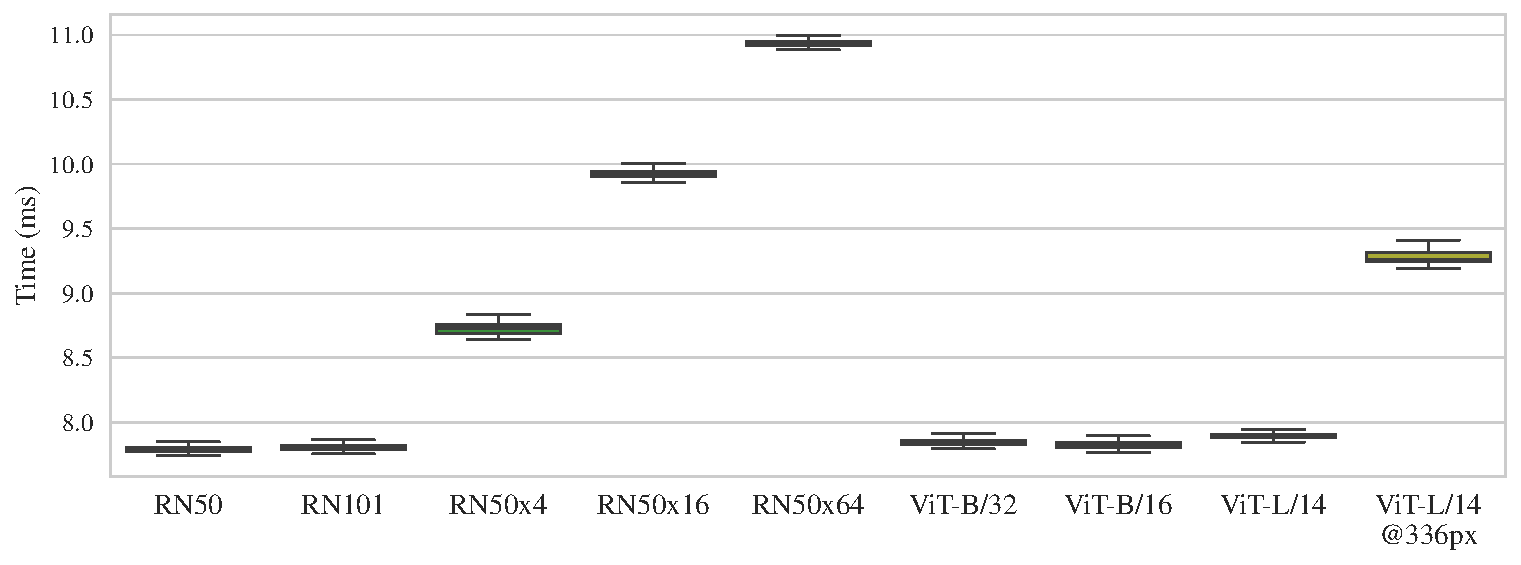
\includegraphics[width=\textwidth]{images/full_transform.pdf}\vspace{-15pt}
    \caption{Preprocessing times before optimizations.}\vspace{15pt}
    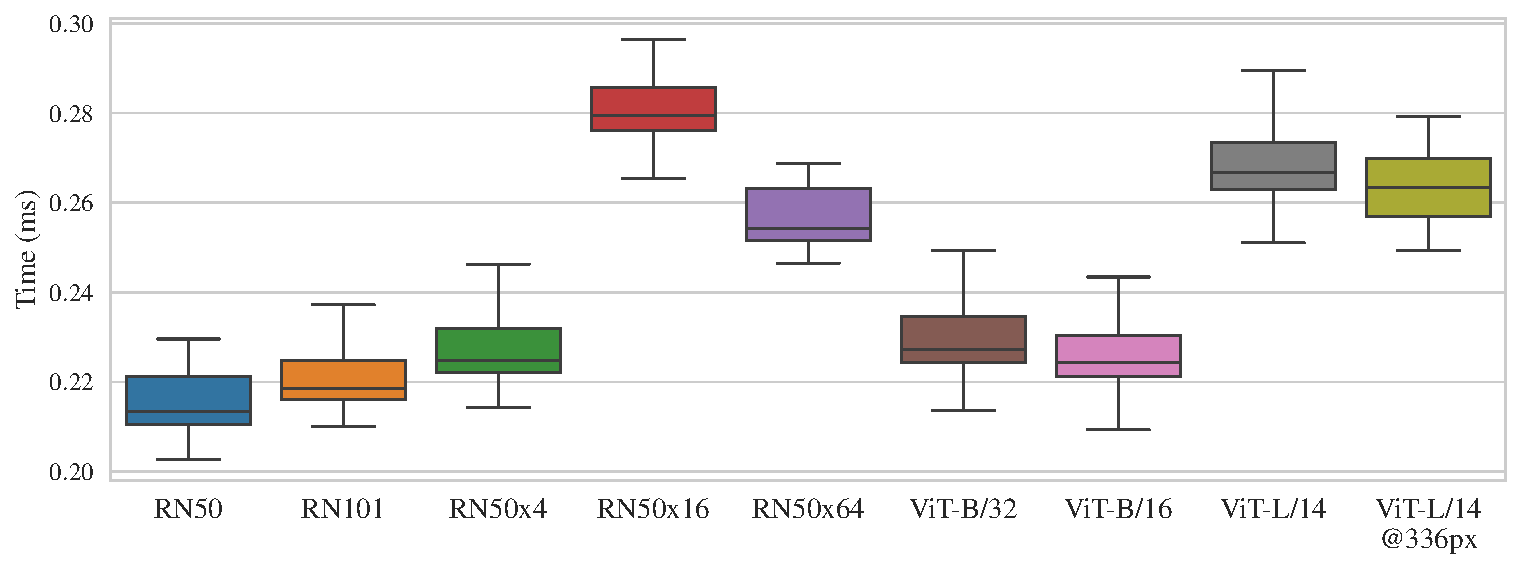
\includegraphics[width=\textwidth]{images/fast_transform.pdf}\vspace{-15pt}
    \caption{Preprocessing times after optimizations.}
    \label{fig:preprocessing-time-improvement}
\end{figure}

These modifications are available on \url{https://github.com/pulkitgoyal56/CLIP/tree/preprocess-tweaks}.
